\documentclass{beamer}

\usepackage[utf8]{inputenc}
\usepackage{default}

\title{All colours are beautiful}
\institute{MetaMeute}

\usetheme{Luebeck}

\begin{document}
\begin{frame}
 \maketitle
\end{frame}

\section{Bezugsquellendiskussion}
\begin{frame}
\begin{itemize}
 \item Angebote einholen
 \item Geldtransferkosten (Klassische Überweisung)
 \item Einfuhrumsatzsteuer
 \item Vor der Bestellung: Drei Wege Handshake
\end{itemize}
\end{frame}

\section{Aufbau}
\subsection{Strom}
\begin{frame}
\begin{figure}[h]
 \centering
 \includegraphics[width=5cm,keepaspectratio=true]{./WS2812B_CloseUp.png}
\end{figure}

\begin{description}
\item[Versorgung] 5V
\item[Max. Strom]
\item[Logic Level] Low  $<$ 0.3$\cdot$VDD, 0.7$\cdot$VDD $<$ High
\end{description}

\end{frame}

\subsection{Protokoll}
\begin{frame}
\begin{center}
 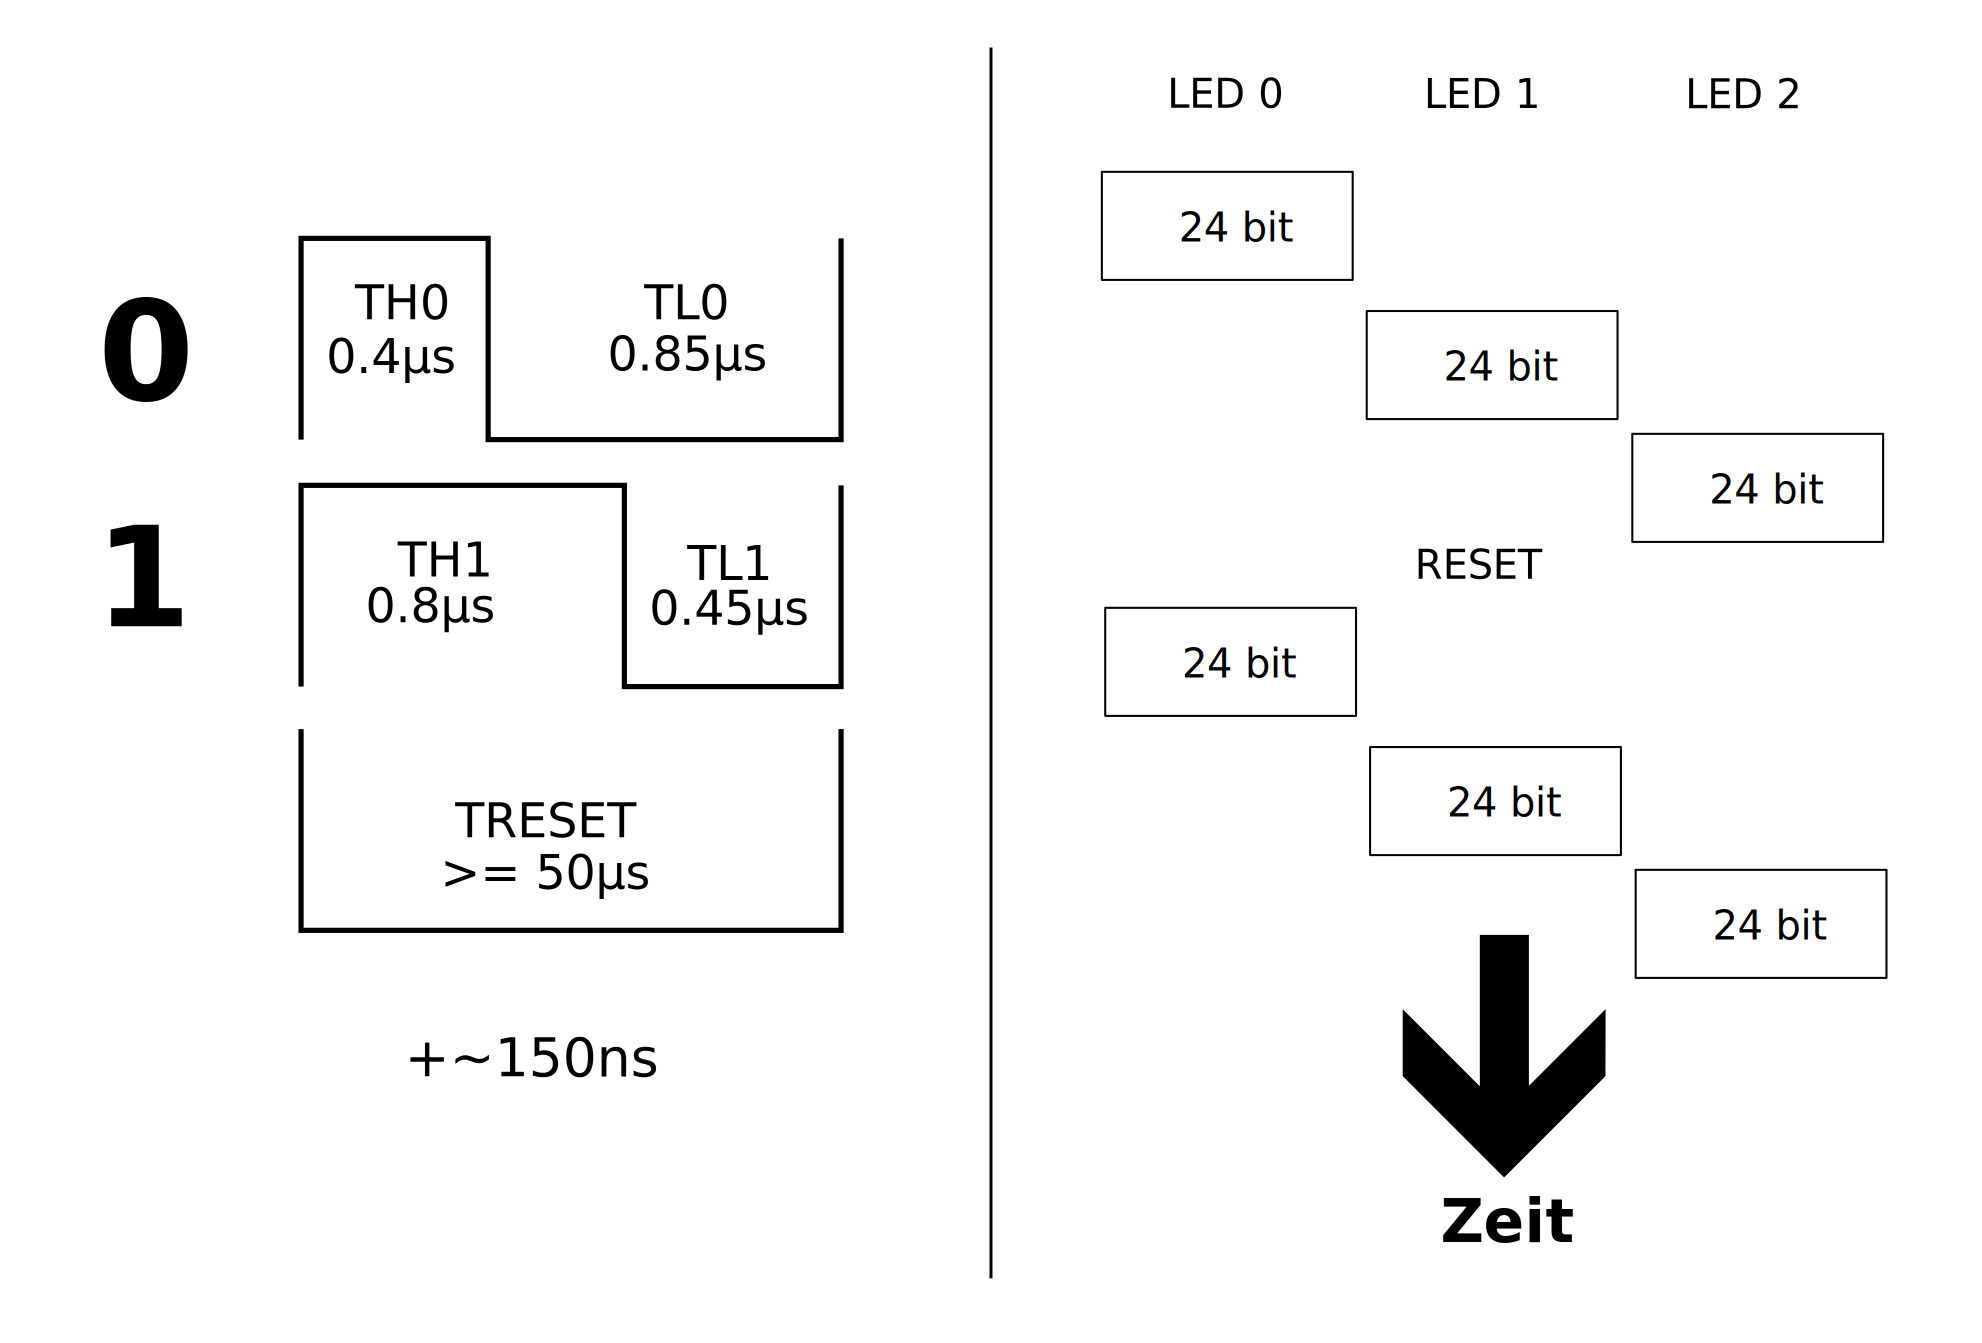
\includegraphics[width=11cm]{protokoll}
\end{center}
\end{frame}

\section{Ansteuerung}
\subsection{Arduino}
\begin{frame}{Arduino}
\begin{figure}[h]
 \centering
 Hier könnte ihre Werbung stehen
\end{figure}
\begin{itemize}
 \item Anfängerorientiertes I/O Board
 \item Hauptsächlich AVR Chips
 \item Viele Varianten, umfangreiche Libraries

\end{itemize}
\end{frame}

\subsection{FTDI}
\begin{frame}{FTDI}
\begin{figure}[h]
 \centering
 Hier könnte ihre Werbung stehen
\end{figure}
\begin{itemize}
 \item Seriell to USB Converter
 \item 3V und 5V Logic
 \item Programmierer für Arduinos, AVRs und Stromversorgung
\end{itemize}

\end{frame}


\subsection{VoCore}
\begin{frame}{VoCore}
\begin{figure}[h]
 \centering
 Hier könnte ihre Werbung stehen
\end{figure}
\begin{itemize}
 \item 2.5x2.5cm SoC (360MHz, 32MB) mit OpenWrt
 \item Günstig, mit Wifi 802.11n, Ethernet 10/100MHz
 \item Unterstützt USB, UART, SPI, I2C, Ethernet mit 28 GPIOs
\end{itemize}
\end{frame}

\section{Projekte}
\subsection{Freifunk-Logo}
\begin{frame}
\end{frame}

\subsection{Musik-Visualisierung}
\begin{frame}
\end{frame}

\subsection{Lichtquelle}
\begin{frame}
\end{frame}

\section{Quellen}
\begin{frame}
 Hier Links zum git
\begin{itemize}
 \item https://github.com/Gnoxter/Nook15-Vortrag
 \item https://github.com/Gnoxter/StripEvents
\end{itemize}
\end{frame}


\end{document}
